\documentclass[10pt, a4paper]{article}

%%%%%%%%%%%%%%
%  Packages  %
%%%%%%%%%%%%%%


\usepackage{page_format}
\usepackage{special}
\usepackage{hyperref}
\usepackage{tikz}
\usepackage[compat=1.1.0]{tikz-feynman}
%----------------------------------------------------------------------
%\usepackage{amssymb} % Mathematical fonts.
%\usepackage{amsfonts} % Mathematical fonts.
\usepackage[nice]{nicefrac} % Nicer fractions
\usepackage{braket} % Dirac Notation.
\usepackage{bbm} % More bold fonts.
%\usepackage{mathrsfs} % Mathematical fonts.
\usepackage{esint} % Integrals
\usepackage{cancel} % Allows to scratch expressions.
\usepackage{mathtools} % Tools for math formating.
\usepackage{slashed} % Allows to slash individual characters.
\usepackage{xargs} % Better handling of optional arguments for commands
%----------------------------------------------------------------------
%\usepackage{lmodern} % Fonts.
\usepackage{feyn} % Feynman Diagrams in mathmode

%%%%%%%%%%%%%%%%%%%%%%%%%%%
% Mathématiques et physique
%%%%%%%%%%%%%%%%%%%%%%%%%%%%
% SI Units -----------------------
% The package 'siunitx' causes unresolved crashes (as of 22/08/31)
\newcommand{\ampere}{\text{A}}
\newcommand{\bell}{\text{B}}
\newcommand{\celsius}{\degree\text{C}}
\newcommand{\coulomb}{\text{C}}
\newcommand{\degree}{\,^{\circ}}
\newcommand{\farad}{\text{F}}
\newcommand{\electro}{\text{e}}
\newcommand{\gram}{\text{g}}
\newcommand{\henry}{\text{H}}
\newcommand{\hertz}{\text{Hz}}
\newcommand{\hour}{\text{h}}
\newcommand{\joule}{\text{J}}
\newcommand{\kelvin}{\text{K}}
\newcommand{\meter}{\text{m}}
\newcommand{\minute}{\text{m}}
\newcommand{\mole}{\text{mol}}
\newcommand{\newton}{\text{N}}
\newcommand{\ohm}{\Omega}
\newcommand{\pascal}{\text{Pa}}
\newcommand{\rad}{\text{rad}}
\newcommand{\second}{\text{s}}
\newcommand{\tesla}{\text{T}}
\newcommand{\torr}{\text{Torr}}
\newcommand{\volt}{\text{V}}
\newcommand{\watt}{\text{W}}
%
\newcommand{\tera}{\text{T}}
\newcommand{\giga}{\text{G}}
\newcommand{\mega}{~\text{M}}
\newcommand{\kilo}{~\text{k}}
\newcommand{\deci}{\text{d}}
\newcommand{\centi}{\text{c}}
\newcommand{\milli}{\text{m}}
\newcommand{\micro}{\mu}
\newcommand{\nano}{\text{n}}
\newcommand{\pico}{\text{p}}
\newcommand{\femto}{\text{f}}
%
\newcommand{\units}[1]{\text{#1}}
\newcommand{\tothe}[1]{\textsuperscript{#1}}
%
\newcommand{\per}{\text{/}}
%
\newcommand{\Time}[3]{#1\hour~#2\minute~#3\second} % TODO Optional arguments.
\newcommand{\Angle}[3]{#1^{\circ}~#2'~#3''} % TODO Optional arguments.


% Better epsilon -----------------------
\let\oldepsilon\epsilon
\let\epsilon\varepsilon
\let\varepsilon\oldepsilon


% Better \bar -----------------------
\renewcommand{\bar}[1]{\mkern 1.5mu\overline{\mkern-1.5mu#1\mkern-1.5mu}\mkern 1.5mu}


% Équations -----------------------
\newcommand{\al}[1]{\begin{align} #1 \end{align}} % Numbered equation(s),
\newcommand{\eqn}[1]{\begin{align*} #1 \end{align*}} % Number-less equation(s),
\newcommand{\sys}[1]{\begin{dcases*} #1 \end{dcases*}} % System of equations.


% Exponents -----------------------
\newcommand{\Exp}[1]{\text{e}^{#1}}		% e^#
\newcommand{\E}[1]{\times 10^{#1}}		% X 10^#


% Delimiters -----------------------
\newcommand{\p}[1]{\left( #1 \right)}	% (#)
\newcommand{\cro}[1]{\left[ #1 \right]}	% [#]
\newcommand{\abs}[1]{\left| #1\right|}	% |#|
\newcommand{\avg}[1]{\left\langle #1 \right\rangle} % <#>
\newcommand{\acc}[1]{\left\lbrace #1 \right\rbrace} % {#}


% Vectors -----------------------
\newcommand{\ve}[1]{\mathbf{#1}} % Upright bold face.
\newcommand{\vu}[1]{\hat{\ve{#1}}} % Hat vector upright bold face
\newcommand{\tens}{\otimes} % Tensor product
\newcommand{\nablav}{\bm{\nabla}} % Bold gradient


% Trig. functions with automatic formating  -----------------------
\newcommandx{\Sin}[2][1={}]{\text{sin}^{#1}\!\p{#2}}
\newcommandx{\Cos}[2][1={}]{\text{cos}^{#1}\!\p{#2}}
\newcommandx{\Tan}[2][1={}]{\text{tan}^{#1}\!\p{#2}}
\newcommandx{\Csc}[2][1={}]{\text{csc}^{#1}\!\p{#2}}
\newcommandx{\Sec}[2][1={}]{\text{sec}^{#1}\!\p{#2}}
\newcommandx{\Cot}[2][1={}]{\text{cot}^{#1}\!\p{#2}}
\newcommandx{\Arcsin}[2][1={}]{\text{arcsin}^{#1}\!\p{#2}}
\newcommandx{\Arccos}[2][1={}]{\text{arccos}^{#1}\!\p{#2}}
\newcommandx{\Arctan}[2][1={}]{\text{arctan}^{#1}\!\p{#2}}
\newcommandx{\Sinh}[2][1={}]{\text{sinh}^{#1}\!\p{#2}}
\newcommandx{\Cosh}[2][1={}]{\text{cosh}^{#1}\!\p{#2}}
\newcommandx{\Tanh}[2][1={}]{\text{tanh}^{#1}\!\p{#2}}


% Matrices -----------------------
\newcommand{\mat}[1]{\begin{bmatrix} #1 \end{bmatrix}} % Matrices with hooks.
\newcommand{\pmat}[1]{\begin{pmatrix} #1 \end{pmatrix}} % Matrices with parentheses.
\newcommand{\deter}[1]{\abs{\begin{matrix} #1 \end{matrix}}} % Determinant.
\newcommandx{\mO}[2][1={}, 2={}]{ \def\temp{#2}\ifx\temp\empty\ve{O}_{#1}\else\ve{O}_{#1\times #2}\fi}% Zero matrix.
\newcommandx{\mI}[2][1={}, 2={}]{ \def\temp{#2}\ifx\temp\empty\ve{I}_{#1}\else\ve{O}_{#1\times #2}\fi}%  Identity matrix.
\newcommand{\Det}[1]{\text{det}\p{#1}} % det(#)
\newcommand{\Tr}[1]{\text{Tr}\p{#1}} % Tr(#)


% Derivatives -----------------------
\newcommand{\D}{\text{d}} % Differential 'd'.
\newcommandx{\dd}[3][1={},3={}]{\frac{\D^{#3}#1}{\D{#2}^{#3}}} % Total derivative according to #2, #1 is the function and #3 is the order.
\newcommand{\del}{\partial} % Partial 'd'.
\newcommandx{\ddp}[3][1={},3={}]{\frac{\del^{#3}#1}{\del{#2}^{#3}}} % Dérivée partielle selon #2, #1 est la fonction est #3 est l'ordre.
\newcommand{\eval}[1]{\left. {#1} \right|} % Bar on the right of expression.
\newcommand{\delbar}{\slashed{\del}} % Partial Inexact differential.
\newcommand{\dbar}{\dj}% Inexact differential.


% Integrals -----------------------
\newcommand{\intinf}{\int\displaylimits_{-\infty}^{\infty}} % From -00 to 00.
\newcommandx{\Int}[2][1={},2={}]{\int\displaylimits_{#1}^{#2}} % Faster bounded integrals.


% Complex numbers -----------------------
\renewcommand{\Re}[1]{\text{Re}\acc{#1}} % Re{#}
\renewcommand{\Im}[1]{\text{Im}\acc{#1}} % Im{#}


% Sets -----------------------
\newcommand{\N}{\mathbbm{N}} % Natural numbers.
\newcommand{\Z}{\mathbbm{Z}} % Integers.
\newcommand{\Q}{\mathbbm{Q}} % Rational numbers.
\newcommandx{\R}[1][1={}]{\mathbbm{R}^{#1}} % Real numbers.
\newcommandx{\C}[1][1={}]{\mathbbm{C}^{#1}} % Complex numbers.
\newcommandx{\F}[1][1={}]{\mathbbm{F}^{#1}} % Some field.
\newcommand{\M}[3]{\mathbb{M}_{#1\times#2}(#3)}	% Matrices.
\newcommand{\Po}[2]{\mathbb{P}_{#1}(#2)} % Polynomials.
\newcommand{\Lin}{\mathbb{L}} % Linear maps.


% Constants and physical symbols -----------------------
\newcommand{\eo}{\epsilon_0} % epsilon 0.
\renewcommand{\L}{\mathcal{L}} % Lagrangian.

\usepackage{slashed}

% References
\usepackage{biblatex}
\addbibresource{ref.bib}
\usetikzlibrary{positioning}


%%%%%%%%%%%%
%  Colors  %
%%%%%%%%%%%%
% ! EDIT HERE !
\colorlet{chaptercolor}{red!70!black} % Foreground color.
\colorlet{chaptercolorback}{red!10!white} % Background color

%%%%%%%%%%%%%%
% Page titre %
%%%%%%%%%%%%%%%
\title{Homework 2} % Title of the assignement.
\author{\PA} % Your name(s).
\teacher{Yin-Chen He and Timothy Hsieh} % Your teacher's name.
\class{Quantum Matter} % The class title.

\university{Perimeter Institute for Theoretical Physics} % University
\faculty{Perimeter Scholars International} % Faculty
%\departement{<Departement>} % Departement
\date{\today} % Date.


%%%%%%%%%%%%%%%%%%%%%%
% Begin the document %
%%%%%%%%%%%%%%%%%%%%%%
\begin{document}

% Make the title page.
\maketitlepage

% Make table of contents
\maketableofcontents

% Assignment starts here ----------------------------

\footnotesize{

\section{2D CFT and the 1D Transverse-Field Ising Chain}

\begin{enumerate}
  \item[(a)] We want to study the 2D CFT that underlies the quantum critical behavior at the 1D transverse field Ising model (TFIM) phase transition. Putting this 2D CFT on the plane, we have a natural parametrization of the fields with the complex variable $z = x+iy$ and its conjugate $\bar{z}$. Each primary field is characterized by the way it transforms under a dilation $z \to \lambda z$ with factor $\lambda \in \mathbb{R}^+$ and rotation $z \to e^{i \theta} z$ at angle $\theta \in [0, 2\pi)$. For a primary field $\varphi_\alpha$, these transformations respectively have the effects $\varphi_\alpha(z) \to \lambda^{\Delta_\alpha}\varphi_{\alpha}(\lambda z)$ and $\varphi_{\alpha}(z) = e^{- i \theta S_\alpha} \varphi_{\alpha}(e^{i \theta} z)$ where $\Delta_\alpha$ is the scaling dimension and $S_\alpha$ is the spin of the primary. Using the properties of the Virasoro algebra, we can construct conformal towers from each primary by regrouping them with their descendants. \\
  
  It is possible to use quantization to extract the CFT data $\{\Delta_\alpha, S_\alpha, c\}$ where $c$ is the central charge. We start by applying a Weyl transformation to the complex plane to bring it to a cylinder: each concentric circle with $z=0$ at its center is mapped to a circle of length $L$ at different heights on the cylinder. We then quantize the CFT by associating a Hilbert space to each circle. The Hamiltonian $H^{\rm CFT}$ connecting these Hilbert spaces at different heights (times) is connecting circles of different radii in the original space and is related to the Dilation operator through an affine transformation. In this quantization, there is a correspondence between each CFT operator and states on a circle Hilbert space. The states $\ket{\varphi_\alpha}$ corresponding to operators with well-defined spins and scaling dimensions (more general than primaries and descendants, the stress-energy tensor is included but is quasi-primary in 2D) are accessible through the spectrum of the dilation operator and indirectly through the spectrum $\{E_{\alpha} = \frac{2\pi}{L} (\Delta_\alpha - \frac{c}{12})\}$ of $H^{\rm CFT}$. \\

  We can construct a sequence of finite size Hamiltonians (finite dimensional Hilbert space) that approach $H^{\rm CFT}$ for the 2D Ising CFT as size increases. The most natural family of Hamiltonians achieving this is the TFIM Hamiltonian given by 
  \begin{align*}
    H=-\sum_{i=1}^L Z_i Z_{i+1}-\sum_{i=1}^L X_i
  \end{align*}
  where $Z_i, X_i$ are Pauli operators acting at site $i$ of a system with $L \in \mathbb{N}$ sites associated to a two-dimensionnal Hilbert space. We use the identification $L \sim 0$ to have the model defined on a circle and eventually have its Hilbert space match the CFT Hilbert space in the $L \to \infty$ limit. We note that the values of transverse field and ferromagnetic coupling are set equal to $1$ so that the Hamiltonian is associated with the quantum critical point of the TFIM. From $H$, we can build operators that produce (in the $L \to \infty$ limit) states corresponding to descendants when acting on states corresponding to primaries. These operators are Fourier modes of $H$ and are expressed at 
  \begin{align*}
    H_n = -\frac{N}{2 \pi} \sum_{j=1}^L \exp \left(\mathrm{i}(j+1 / 2) n \frac{2 \pi}{N}\right) Z_j Z_{j+1}-\frac{N}{2 \pi} \sum_{j=1}^L \exp \left(\mathrm{i} j n \frac{2 \pi}{N}\right) X_j
  \end{align*}
  where $N = L$ is the number of modes. This operator is affected by finite size effects and the connection between finite size approximations of descendants and primary states is made stronger with the operator 
  \begin{align*}
    O_n=\frac{H_n+H_{-n}}{2} \to_{L\to \infty} \frac{L_n^{\rm C F T}+\bar{L}_{-n}^{\rm C F T}+L_{-n}^{\rm C F T}+\bar{L}_n^{\rm C F T}}{2} \quad \text { for } n>0
  \end{align*}
  where $\{L_n^{\rm CFT}, \bar{L}_{n}^{\rm CFT}\}$ of Virasoro algebra operators. For a state $\ket{\varphi}$ corresponding to a primary, the Virasoro operators $L_{n}^{\rm CFT}, \bar{L}_{n}^{\rm CFT}$ for $n > 0$ act as $\bar{L}_{n}^{\rm CFT} \ket{\varphi} = L_{n}^{\rm CFT} \ket{\varphi} = 0$. This is the defining property of primary states. Going in the opposite direction, every descendant state can be reached from primary states by acting $L_{-n}^{\rm CFT}, \bar{L}_{-n}^{\rm CFT}$. We note that $L_{-1}^{\rm CFT}, L_{-2}^{\rm CFT}$ (resp. $\bar{L}_{-1}^{\rm CFT}, \bar{L}_{-2}^{\rm CFT}$) generate the subalgebra $L_{-n}^{\rm CFT}$ (resp. $\bar{L}_{-n}^{\rm CFT}$) implying that $n=1, 2$ operators are sufficient to generate all the conformal towers. The scaling dimension $\Delta_{\varphi'}$ of the descendant state $\ket{\varphi'}$ of the primary state $\ket{\varphi}$ with scaling dimension $\Delta_\varphi$ is such that $\Delta_{\varphi'} - \Delta_\varphi \in \mathbb{N}$. \\
  
  In what follows we describe a criterion to identify \textit{approximate} primaries and associate them to descendants in the spectrum of $H$. We start by defining the projector
  \begin{align*}
    \Gamma_{\varphi} \equiv \sum_{\varphi_\alpha: E_\alpha<E_{\varphi}}\left|\varphi_\alpha\right\rangle\left\langle\varphi_\alpha\right|
  \end{align*}
  which projects on the subspace of spaned by energy eigenstates below $E_\varphi$ (the energy of the primary corresponding to the projector). Then we use "$\bar{L}_{n}^{\rm CFT} \ket{\varphi} = L_{n}^{\rm CFT} \ket{\varphi} = 0 \iff \ket{\varphi}$ is primary" to write 
  \begin{align*}
    \ket{\varphi} \text{ is primary} \implies \Gamma_{\varphi} O_n \ket{\varphi} &= \sum_{\varphi_\alpha: E_\alpha<E_{\varphi}}\left|\varphi_\alpha\right\rangle\left\langle\varphi_\alpha\right|\frac{L_n^{\rm C F T}+\bar{L}_{-n}^{\rm C F T}+L_{-n}^{\rm C F T}+\bar{L}_n^{\rm C F T}}{2} \ket{\varphi} \\
    &=  \sum_{\varphi_\alpha: E_\alpha<E_{\varphi}}\left|\varphi_\alpha\right\rangle\left\langle\varphi_\alpha\right|\frac{\bar{L}_{-n}^{\rm C F T}+L_{-n}^{\rm C F T}}{2} \ket{\varphi}, \quad \text{$\ket{\varphi}$ is primary}\\
    &= \sum_{\varphi_\alpha: E_\alpha<E_{\varphi}}\left|\varphi_\alpha\right\rangle\left\langle\varphi_\alpha\right| \frac{\ket{\varphi'} + \ket{\varphi''}}{2}, \quad \text{$\ket{\varphi'} = L_{-n}^{\rm C F T} \ket{\varphi}$, $\ket{\varphi''} = \bar{L}_{-n}^{\rm C F T} \ket{\varphi}$ (descendants with $E_{\varphi'} = E_{\varphi''} > E_{\varphi}$)}\\
    &= 0 
  \end{align*}
  where the energies of the descendant states $\ket{\varphi'}$ and $\ket{\varphi''}$ are both equal to $E_{\varphi'} = E_{\varphi''} = \frac{2\pi}{L} (\Delta_\alpha + n - \frac{c}{12}) > E_\varphi$ (but their spins are different making them distinguishable \textcolor{red}{add reference to paper}). 
  \newpage 
  The reverse direction of this implication is established with 
  \begin{align*}
    0 &= \Gamma_{\varphi} O_n \implies 0 = \sum_{\varphi_\alpha: E_\alpha<E_{\varphi}}\left|\varphi_\alpha\right\rangle\left\langle\varphi_\alpha\right|\frac{L_n^{\rm C F T} + \bar{L}_n^{\rm C F T}}{2} \ket{\varphi} \implies \ket{\varphi} \text{ is primary}
  \end{align*}
  where we removed the $L_{-n}^{\rm C F T}$ and $\bar{L}_{-n}^{\rm C F T}$ terms because they increase the energy beyond the projector scope (this is true if $\ket{\varphi}$ is a primary \textit{or} a descendant). The last implication is supported by the fact acting $L_n^{\rm C F T}, \bar{L}_n^{\rm C F T}$ on a descendant will lower its energy (possibly to a primary state) to the scope of the projector leading to a non-zero contribution. Only primaries escape the scope of the projector because they are mapped to zero directly by $L_n^{\rm C F T}, \bar{L}_n^{\rm C F T}$.\\
  
  In the finite size spectrum of $H$, the approximate primaries can be found by numerically computing the norm $\epsilon^{(n)}_\varphi \equiv |\Gamma_{\varphi} O_n\ket{\varphi}|$. This norm is zero in the limit $L\to \infty$ iff we have a primary state. For finite $L$, we relax the zero norm condition to a small norm condition. More precisely, we introduce a threshold $\epsilon_{\rm max}$ and declare an eigenstate of $H$ "primary candidate" iff $\epsilon \equiv \epsilon^{(1)}_\varphi + \epsilon^{(2)}_\varphi \leq \epsilon_{\rm max}$. 
  \item[(b)] Using the criterion described in (a) we can extract primary candidates for the TFIM CFT. We use a sparse exact diagonalization Python code to find the $22$ lowest energy states in the spectrum of $H$ at size $L = 16$ and look for the three lowest primary states. The scaling dimension obtained after shifting and rescaling the spectrum of $H$ (see (c)) are associated with the values of $\epsilon$ displayed in Table \ref{spectrum_eps}. We note that only the first three states meet the condition $\epsilon \leq 10^{-12}$ and we associate them with the primary operators $I$ (identity) $\sigma$ and $\varepsilon$. 
  \begin{table}
    \centering
        \begin{minipage}{.5\linewidth}
          \flushright
          \begin{tabular}{lr}
            \toprule
            $\Delta$ & $\log \epsilon$ \\
            \midrule
            0.0000 & -$\infty$\\
            0.1265 & -32.83 \\
            1.0097 & -31.09 \\
            1.1314 & -1.00 \\
            1.1314 & -1.08 \\
            2.0000 & 0.28 \\
            2.0000 & 0.15 \\
            2.0000 & -1.00 \\
            2.0000 & -0.19 \\
            2.0976 & 0.70 \\
            2.0976 & 0.84 \\
            \bottomrule
            \end{tabular}
        \end{minipage}%
        \begin{minipage}{.5\linewidth}
          \flushleft
          \begin{tabular}{lr}
            \toprule
            $\Delta$ & $\log \epsilon$ \\
            \midrule
            2.1362 & -0.69 \\
            2.9328 & 0.95 \\
            2.9328 & 1.30 \\
            2.9328 & 0.95 \\
            2.9328 & 1.01 \\
            2.9881 & 1.47 \\
            2.9881 & 1.47 \\
            2.9903 & 0.34 \\
            3.1024 & -0.15 \\
            3.1024 & 0.43 \\
            3.1024 & 0.10 \\
            \bottomrule
            \end{tabular}
        \end{minipage} 

      \caption{Approximate $H^{\rm CFT}$ spectrum and associated primary test $\epsilon$ for the $22$ lowest scaling dimension states at size $L=16$ \label{spectrum_eps}}
  \end{table}
  
  \item[(c)] The TFIM Hamiltonian is related in the $L\to \infty$ limit to the CFT Hamiltonian by the affine transformation $H^{\rm CFT} = a H  + b$ for real constants $a, b$. At finite size, we can determine the values of $a, b$ leading to an optimal agreement between the eigenvalues of the low energy states and expected scaling dimensions. We first note that the ground state $\ket{0}$ (with $H \ket{0} = E_0 \ket{0}$) has scaling dimension $\Delta_I = 0$ since it corresponds to the identity $I$. We choose $b = -a E_0$ to shift the eigenvalue of $\ket{0}$ to $0$. At this point we have $H^{\rm CFT} \approx a (H  - E_0)$. To fix $a$ we use the fact $L^{\rm CFT}_{-2} \ket{0}$ (resp. $\bar{L}^{\rm CFT}_{-2} \ket{0}$) is a state $\ket{I, 2}$ (resp. $\ket{\bar{I, 2}}$) with scaling dimension $\Delta_{2}^{I} = 0 + 2$ (shifted by $2$ from $\Delta_I$). To produce an approximation of the effect of $L_{-2}^{\rm CFT}$ at finite size, we use $O_2$ and write 
  \begin{align*}
    O_2 \ket{0} \approx \frac{L_2^{\rm C F T}+\bar{L}_{-2}^{\rm C F T}+L_{-2}^{\rm C F T}+\bar{L}_2^{\rm C F T}}{2} \ket{0} = \frac{\bar{L}_{-2}^{\rm C F T}+L_{-2}^{\rm C F T}}{2} \ket{0} = \frac{\ket{I, 2} + \ket{\bar{I, 2}}}{2}.
  \end{align*}
  Since $O_2 \ket{0}$ is a superposition of two eigenstates with the same scaling dimension (and same energy), it is also an eigenstate of $H$. Acting $H$ on it yields the constraint 
  \begin{align*}
    (H - E_0) O_2 \ket{0} \approx \frac{1}{a} \times H^{\rm CFT} O_2 \ket{0} = \frac{1}{a} \times \frac{2\Delta_2^I}{2}(O_2 \ket{0}) \implies \frac{1}{a} = \frac{|(H - E_0) O_2 \ket{0}|}{\Delta_2^I|O_2 \ket{0}|}
  \end{align*}
  where we chose $a > 0$ to ensure positive scaling dimensions (the spectrum is bounded from below implying the shifted spectrum is positive). This way to calculate $a$ can be implemented numerically. We find the values $a \approx 1.2877$ and $b = 26.2741$. 
  
  \item[(d)] The scaling dimensions extracted from the shifted and rescales Hamiltonian (c) are presented in Table. \ref{spectrum_eps}. For the previously identified primaries (see (b)), the scaling dimensions match the analytical expectations. Explicitly, we have $\Delta_{\sigma} = 0.1265$ (close to the exact value $\Delta_{\sigma} = 1/8$) and $\Delta_{\varepsilon} = 1.0097$ (close to the exact value $\Delta_{\varepsilon} = 1$). 
  \newpage
  \item[(e)] Table \ref{crit_exp} presents a comparison of the exact value of Ising critical exponents \cite{crit_exp} of the 1+1D TFIM phase transition. We see that the calculated exponents approach the exact ones as the system size is increased. 
  \begin{table}
    \centering
    \begin{tabular}{lrrrrrr}
      \toprule
       & $\alpha$ & $\beta$ & $\gamma$ & $\delta$ & $\eta$ & $\nu$ \\
      \midrule
      Exact & 0.000 & 0.125 & 1.750 & 15.000 & 0.250 & 1.000 \\
      $L=16$ & -0.020 & 0.128 & 1.892 & 14.810 & 0.253 & 1.010 \\
      $L=18$ & -0.020 & 0.127 & 1.888 & 14.848 & 0.252 & 1.008 \\
      \bottomrule
      \end{tabular}

      \caption{Calculation of the approximative critical exponents of the 1+1D TFIM phase transition using the approximative scaling dimensions $\Delta_{\sigma}$ and $\Delta_{\varepsilon}$ for two finite system size $L=16$ and $L=18$. The exact values for these exponents are known and compared with the approximative results to show an improvement of the agreement with increasing system size. The expression in terms of primary scaling dimensions and exact values for these exponents can be found at \cite{crit_exp}. \label{crit_exp}}
  \end{table}
  \item[(f)] Using the operators $O_n$ for $n =1, 2$ we can obtain states corresponding to descendants in the conformal towers of the primaries ($I, \sigma, \varepsilon$) found in (b). For $I$ we already studied a descendant $O_2\ket{0}$ with scaling dimension $\Delta_2^I$ in (c). We note that $O_1\ket{0}$ has large finite size effects and it is not studied here. To numerically extract approximation of the scaling dimensions $\Delta_{n}^{I, \sigma, \varepsilon}$ of the states $O_n \ket{I, \sigma, \varepsilon}$, we calculate
  \begin{align*}
     \frac{|(a H + b) O_n \ket{I, \sigma, \varepsilon}|}{|O_n \ket{I, \sigma, \varepsilon}|} \approx \frac{| H^{\rm CFT} O_n \ket{I, \sigma, \varepsilon}|}{|O_n \ket{I, \sigma, \varepsilon}|} = \Delta_{n}^{I, \sigma, \varepsilon}. 
  \end{align*}
  The numerical results of this method are presented in Table \ref{des}. Comparing the obtained scaling dimensions with manual integer shifts expected for descendants, we observe deviations of the order of $0.1$ due to finite size effects. 
  \begin{table}
    \centering
    \begin{tabular}{lcccc}
      \toprule
            $n$ & $\Delta_\sigma + n$ & $\Delta_{n}^\sigma$ & $\Delta_\varepsilon + n$ & $\Delta_{n}^\varepsilon$ \\
      \midrule
      $1$ & 1.131 & 1.127 & 2.000 & 2.010 \\
      $2$ & 2.098 & 2.127 & 2.933 & 3.010 \\
      \bottomrule
      \end{tabular}
    \caption{Comparison of the scaling dimsension obtained by acting the operators $O_1$  (resp. $O_2$) on the primary states $\ket{\sigma}$ and $\ket{\varepsilon}$ with the scaling dimensions $\Delta_\sigma$ and $\Delta_\varepsilon$ increased by $1$ (resp. $2$). \label{des}}
  \end{table}
  \item[(g)]  We finally approximate the central charge $c$ of the 1+1D Ising CFT with the finite size operators. As stated in \cite{spinchain}, $c \approx c_L = 2 \bra{I}H_2^{\dagger} H_2 \ket{I}$ (here $H_2$ differs from the expression given above. It is associated with the rescaled and shifted Hamiltonian. Since only the $n=0$ Fourier mode features dependence on the constant shift $b$, the $n=2$ mode corresponding to the adjusted spectrum is obtained by applying the $a$ rescaling). By combining the approximate central charge obtained numerically for different system sizes, we can extrapolate to $L\to \infty$ and compare with the value $c = 1/2$ expected for the 1+1D Ising CFT. The results obtained are presented in Figure \ref{central_c} 
  \begin{figure}
    \centering
    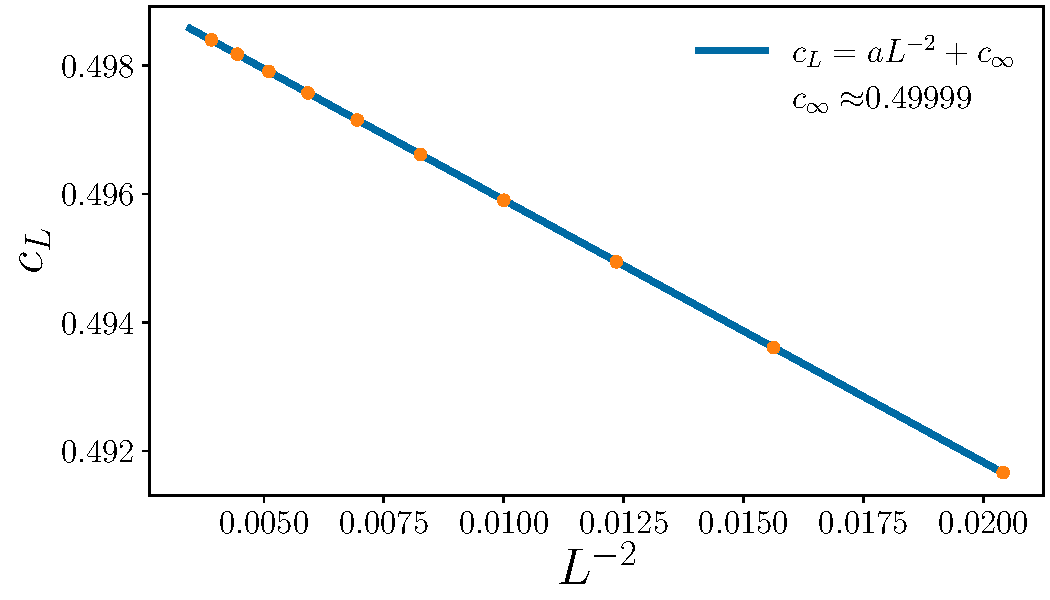
\includegraphics[scale=0.5]{central_charge_fit.pdf}
    \caption{Approximate central charge $c_L = 2 \bra{I}H_2^{\dagger} H_2 \ket{I}$ as a function of $L^{-2}$. A linear fit was used to extrapolate the $L^{-2} \to 0$ ($L\to \infty$) limit of $c_L$. We obtain a value close to the exact $c=1/2$. \textcolor{red}{The formula used in the calculations has no $a$ rescaling for $H_2$ and has $\bra{I}H_2^{\dagger} H_2 \ket{I}/\textcolor{red}{2}$} \label{central_c}.}
  \end{figure}
\end{enumerate}


\section{Acknowledgement}
Thanks to Nikhil for a discussion about quasi primaries. 
}

% References c
\makereferences
%-------------------------------------------------------


%%%%%%%%%%%%%%%%%%%%%%%%
% Terminer le document %
%%%%%%%%%%%%%%%%%%%%%%%%
\end{document}
